%; whizzy section -pdf -initex "pdflatex -ini"
\documentclass[a4paper,11pt,twoside,openright]{report}
\usepackage{hevea}
\usepackage{ifthen}

% true = prints marks signaling the state of the implementation
% false = prints only the ACSL definition, without remarks on implementation.
\newboolean{PrintImplementationRq}
\setboolean{PrintImplementationRq}{false}
%Do not touch the following line. It is used in a Makefile hack to
%produce the ACSL document shipped with the Frama-C distribution.
%--\setboolean{PrintImplementationRq}{true}

% true = remarks about the current state of implementation in Frama-C
% are in color.
% false = they are rendered with an underline
\newboolean{ColorImplementationRq}
%\setboolean{ColorImplementationRq}{true}
\setboolean{ColorImplementationRq}{false}

\usepackage[a4paper=true,pdftex,colorlinks=true,urlcolor=blue,pdfstartview=FitH]{hyperref}

\usepackage[T1]{fontenc}
\usepackage{times}
\usepackage{amssymb}
\usepackage{graphicx}
%\usepackage{tikz}
\usepackage{color}
\usepackage{xspace}
\usepackage{makeidx}
%\usepackage{ulem}
\usepackage[leftbars]{changebar}
\usepackage{alltt}
\makeindex

\newcommand{\experimental}{\textsc{Experimental}}

\newsavebox{\fmbox}
\newenvironment{cadre}
     {\begin{lrbox}{\fmbox}\begin{minipage}{0.98\textwidth}}
     {\end{minipage}\end{lrbox}\fbox{\usebox{\fmbox}}}

\newenvironment{todo}{\begin{quote} 
    \begin{tabular}{||p{0.8\textwidth}}
TODO~:\itshape}{\end{tabular}\end{quote}}

\newenvironment{remark}[1]{\begin{quote}\itshape 
    \begin{tabular}{||p{0.8\textwidth}}
Remarque de {#1}~:}{\end{tabular}\end{quote}}

\newenvironment{oldremark}[1]{\begin{quote}\itshape 
    \begin{tabular}{||p{0.8\textwidth}}
Vieille remarque de {#1}~:
}{
\end{tabular}\end{quote}
}

\newcommand{\keyword}[1]{\texttt{#1}\xspace}

\newcommand{\integer}{\keyword{integer}}
\newcommand{\real}{\keyword{real}}
\newcommand{\boolean}{\keyword{boolean}}
\newcommand{\assert}{\keyword{assert}}
\newcommand{\assume}{\keyword{assume}}
\newcommand{\requires}{\keyword{requires}}
\newcommand{\ensures}{\keyword{ensures}}
\newcommand{\assumes}{\keyword{assumes}}
\newcommand{\assigns}{\keyword{assigns}}
\newcommand{\reads}{\keyword{reads}}
\newcommand{\decreases}{\keyword{decreases}}
\newcommand{\boundseparated}{\keyword{{\textbackslash}bound\_separated}}
\newcommand{\Exists}{\keyword{{\textbackslash}exists}~}
\newcommand{\Forall}{\keyword{{\textbackslash}forall}~}
\newcommand{\freed}{\keyword{{\textbackslash}freed}}
\newcommand{\fresh}{\keyword{{\textbackslash}fresh}}
\newcommand{\fullseparated}{\keyword{{\textbackslash}full\_separated}}
\newcommand{\Max}{\keyword{max}}
\newcommand{\nothing}{\keyword{{\textbackslash}nothing}}
\newcommand{\numof}{\keyword{num\_of}}
\newcommand{\offsetmin}{\keyword{{\textbackslash}offset\_min}}
\newcommand{\offsetmax}{\keyword{{\textbackslash}offset\_max}}
\newcommand{\old}{\keyword{{\textbackslash}old}}
\newcommand{\at}{\keyword{{\textbackslash}at}}

\newcommand{\If}{\keyword{if}~}
\newcommand{\Then}{~\keyword{then}~}
\newcommand{\Else}{~\keyword{else}~}
\newcommand{\For}{\keyword{for}~}
\newcommand{\While}{~\keyword{while}~}
\newcommand{\Do}{~\keyword{do}~}
\newcommand{\Let}{\keyword{\textbackslash{}let}~}

\newcommand{\struct}{\keyword{struct}}
\newcommand{\union}{\keyword{union}}
\newcommand{\inter}{\keyword{inter}}
\newcommand{\typedef}{\keyword{typedef}}
\newcommand{\result}{\keyword{{\textbackslash}result}}
\newcommand{\separated}{\keyword{{\textbackslash}separated}}
\newcommand{\sizeof}{\keyword{sizeof}}
\newcommand{\strlen}{\keyword{{\textbackslash}strlen}}
\newcommand{\Sum}{\keyword{sum}}
\newcommand{\valid}{\keyword{{\textbackslash}valid}}
\newcommand{\validrange}{\keyword{{\textbackslash}valid\_range}}
\newcommand{\offset}{\keyword{{\textbackslash}offset}}
\newcommand{\blocklength}{\keyword{{\textbackslash}block\_length}}
\newcommand{\baseaddr}{\keyword{{\textbackslash}base\_addr}}
\newcommand{\comparable}{\keyword{{\textbackslash}comparable}}

\newcommand{\N}{\ensuremath{\mathbb{N}}}
\newcommand{\ra}{\ensuremath{\rightarrow}}


% BNF grammar

\newif\ifspace
\newif\ifnewentry
\newcommand{\addspace}{\ifspace \; \spacefalse \fi}
\newcommand{\term}[1]{\addspace\hbox{\texttt{#1}} \spacetrue}
\newcommand{\nonterm}[1]{%
\addspace\hbox{\textsl{#1}\ifnewentry\index{#1@\textsl{#1}!non-terminal}\fi}\spacetrue}
\newcommand{\repetstar}{^*\spacetrue}
\newcommand{\repetplus}{^+\spacetrue}
\newcommand{\repetone}{^?\spacetrue}
\newcommand{\lparen}{\addspace(}
\newcommand{\rparen}{)}
\newcommand{\orelse}{\addspace\mid\spacetrue}
\newcommand{\sep}{ \\[2mm] \spacefalse\newentrytrue}
\newcommand{\newl}{ \\ & & \spacefalse}
\newcommand{\alt}{ \\ & \mid & \spacefalse}
\newcommand{\is}{ & ::= & \newentryfalse}
\newenvironment{syntax}{$$\begin{array}{rrll}\spacefalse}{\end{array}$$}
\newcommand{\synt}[1]{$\spacefalse#1$}
\newcommand{\emptystring}{\epsilon}
\newcommand{\below}{See\; below}

% colors

\definecolor{darkgreen}{rgb}{0, 0.5, 0}

% theorems

\newtheorem{example}{Example}[chapter]

%%% Local Variables:
%%% mode: latex
%%% TeX-PDF-mode: t
%%% TeX-master: "main"
%%% End:


\setlength{\textheight}{240mm}
\setlength{\topmargin}{-10mm}
\setlength{\textwidth}{160mm}
\setlength{\oddsidemargin}{0mm}
\setlength{\evensidemargin}{0mm}
\newcommand{\version}{1.4}

\renewcommand{\textfraction}{0.01}
\renewcommand{\topfraction}{0.99}
\renewcommand{\bottomfraction}{0.99}

\usepackage{fancyhdr}
\pagestyle{fancyplain}
\renewcommand{\footrulewidth}{0.4pt}
\addtolength{\headheight}{2pt}
\addtolength{\headwidth}{1cm}
\renewcommand{\chaptermark}[1]{\markboth{#1}{}}
\renewcommand{\sectionmark}[1]{\markright{\thesection\ #1}}
\lhead[\fancyplain{}{\bfseries\thepage}]{\fancyplain{}{\bfseries\rightmark}}
\chead{}
\rhead[\fancyplain{}{\bfseries\leftmark}]{\fancyplain{}{\bfseries\thepage}}
\lfoot{\fancyplain{}{ANSI/ISO C Specification Language}}
\cfoot{}
\rfoot{\fancyplain{}{CAT RNTL project}}

\begin{document}
\sloppy
\hbadness=10000

\begin{titlepage}
\begin{center}

\includegraphics[height=14mm]{cealistlogo.jpg}
\hfill

\includegraphics[height=14mm]{inriasaclaylogo.png}

\vfill

%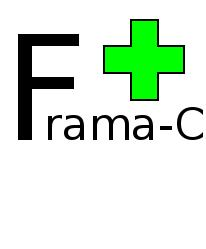
\includegraphics[height=60mm]{FramaC.jpg}
~

\vspace{20mm}

{\Huge\bfseries ACSL: ANSI/ISO C Specification Language}

\bigskip

{\LARGE Preliminary design (version \version, \today)}

\vspace{20mm}

{Patrick Baudin$^1$, Jean-Christophe Filli\^atre$^{4,3}$, Claude March\'e$^{3,4}$,\\ Benjamin Monate$^1$, Yannick Moy$^{2,4,3}$, Virgile Prevosto$^1$}

\medskip

\begin{tabular}{l}
$^1$ CEA LIST, Software Reliability Laboratory, Saclay, F-91191 \\
$^2$ France T\'el\'ecom, Lannion, F-22307 \\
$^3$ INRIA Saclay - \^Ile-de-France, ProVal, Orsay, F-91893 \\
$^4$ LRI, Univ Paris-Sud, CNRS, Orsay, F-91405
\end{tabular}

\vfill


\begin{flushleft}
  This work has been supported by the 'CAT' ANR project
  (ANR-05-RNTL-0030x) and by the ANR CIFRE contract 2005/973.
\end{flushleft}

\end{center}
\end{titlepage}

\clearpage
\label{chap:contents}
\tableofcontents

\chapter*{Foreword}

This is a preliminary design of the ACSL language, a deliverable of
the task 7.2 of the ANR RNTL project CAT
(\url{http://www.rntl.org/projet/resume2005/cat.htm}). In this
project, a reference implementation of ACSL is provided: the Frama-C
platform (\url{http://frama-c.cea.fr}).

This is the version \version{} of ACSL design. Several features may still
evolve in the future. In particular, some features in this document
are considered \emph{experimental}, meaning that their syntax and
semantics is not already fixed.  These features are marked with
\experimental.  They must also be considered as advanced features,
which are not supposed to be useful for a basic use of that
specification language.

\section*{Acknowledgements}

We gratefully thank all the people who contributed to this document:
Sylvie Boldo,
Jean-Louis Cola\c{c}o,
Pierre Cr\'egut,
Pascal Cuoq,
David Delmas,
St\'ephane Duprat,
Arnaud Gotlieb,
Thierry Hubert,
Dillon Pariente,
Pierre Rousseau,
Julien Signoles,
Jean Souyris.

\chapter{Introduction}

This document is a reference manual for ACSL, an acronym for ``ANSI C
Specification Language''. This is a specification language proposed by
the CAT
project\footnote{\url{http://www.rntl.org/projet/resume2005/cat.htm},
  \todo{referer a une page publique en anglais dont la creation a ete
  decide}}, implemented in the \textsc{Frama-C} platform, which aims at
specifying behavioral properties of C source code. The main
inspiration for this language comes from the specification language of
the \textsc{Caduceus} tool~\cite{filliatre04icfem,filliatre07cav} for
deductive verification of behavioral properties of C programs. It is
itself inspired from the \emph{Java Modeling Language} (JML) which
aims at similar goals for Java source code: indeed it aims both at
\emph{runtime assertion checking} and \emph{static verification} using
the \textsc{ESC/Java2} tool~\cite{ESCJava2}, where we aim at 
\emph{static verification} and \emph{deductive verification}.

Going back further in history, JML design was guided by the general
\emph{design-by-contract} principle proposed by Bertrand Meyer, who
took his own inspiration from the concepts of preconditions and
postconditions on a routine, going back at least to Dijkstra, Floyd and
Hoare in the late 60's and early 70's, and originally implemented in
the \textsc{Eiffel} language.

In this document, we assume that the reader has a good knowledge of
the ANSI C programming language~\cite{KR88}.

\section{Organization of this document}

In this preliminary chapter we introduce some definitions and
vocabulary, and discuss generalities about this specification language.

Chapter~\ref{chap:base} presents the specification language itself.

Chapter~\ref{chap:lib} presents additional informations about
\emph{libraries} of specifications.

A detailed table of contents is given on page~\pageref{chap:contents}

\subsection*{Experimental features}

Some features in this document are considered \emph{experimental},
meaning that their syntax and semantics is still under discussion.
These features are marked with \experimental.

They must also be considered as ``advanced features'' which are not
supposed to be useful for a basic use of that specification language.


\section{Glossary}

\begin{description}
\item[pure expressions] \index{pure expression} A C expression is
  called \emph{pure} if it has no side-effect: no assignments, no
  incrementation operator \verb|++| or \verb|--|. Moreover it should
  not contain any function call, even if the called function has no
  side-effect itself.

\item[memory locations and left-values] \index{memory location}
  \index{left value}\index{l-value} A \emph{memory location} is an
  expression which denotes some place in the memory during program
  execution, either on the stack, on the heap, or in the static data
  segment. It can be either a variable identifier or an expression of
  the form $*e$, $e[e]$, $e\verb|.|id$ or $e\verb|->|id$.

  A \emph{left value}, or \emph{l-value} for short, is a memory
  location allowed in the left part of an assignment, that is a
  non-constant memory location.
 
\item[pre-state and post-state]
    \index{pre-state}\index{post-state}
    
    For a given function call, the \emph{pre-state} denotes the
    program's state at the beginning of the call, including the
    current values for the function parameters. the \emph{post-state}
    denotes the program's state at the return of the call.

\item[function behavior] \index{function behavior} \index{behavior}

  A \emph{function behavior} is a set of properties relating the
  pre-state and the post-state for any call to that function.

\item[contract] \index{contract} A \emph{contract} forms a
  specification of a function, consisting of the combination of a
  precondition (an assumption about the pre-state) and a collection
  of behaviors.

\end{description}

\oldremark{Claude}{ce document doit etre illustr� par des
exemples. Toute construction qui ne serait pas illustr�e par un
exemple sera non-retenue.}

\oldremark{Patrick}{utiliser en priorit� les constructions de JML,
ensuite les g�n�raliser lorsque cela a un sens, et en dernier recours,
en cr�er de nouvelles. Il y a peut-�tre des constructions
du C++ ou C\# � utiliser ou � g�n�raliser.
Idem avec les extensions de GCC.}

\section{Generalities about Annotations}

In this document, we consider that annotations are given as comments
written directly into C source files, so
that source files remain compilable\footnote{Other means of attaching
  annotations to source files, without modifying them, are left to user
  tools.}. Those comments must start by \verb|/*@| or \verb|//@|.

\subsection{Kinds of annotations}

\begin{itemize}
\item Global annotations:
  \begin{itemize}
  \item function contract. Such an annotation is inserted just before
    the declaration or the definition of a function.
    See section~\ref{sec:fn-behavior}.

  \item global invariant. This is allowed at the level of global declarations.
    See section~\ref{sec:invariants}.

  \item type invariant. This allows both structure or union
    invariants, and invariants on type names introduced by \typedef.
    See section~\ref{sec:invariants}.

  \item logic specifications: logic type introduction, introduction
    or definition of logic functions or predicates, axioms. Such an
    annotation is placed at the global declarations level.

  \end{itemize}

\item Statement annotations:
  \begin{itemize}
  \item \assert clause, logic label. These are allowed
    everywhere a C label is allowed, or exceptionally just before a
    block closing brace.  
    \oldremark{Claude}{About \assume{} clauses: current
      discussion is that it is not considered as an element of
      specification, so not present here. This should be part of proof
      management done by tools.} 
    \oldremark{Patrick}{En C, seules les
      instructions peuvent �tre �tiquett�es. GCC �tend cela aux
      accolades fermantes des blocs, y compris celle fermant le corps
      de fonction. On peut dire que l'on fait de m�me lorsque l'on
      place des annotations juste avant la fermerture d'un bloc.}
    
  \item loop annotation (invariant, variant, assign clauses) is
    allowed immediately before a loop statement: \For, \While,
    \Do\ldots \While. See Section~\ref{sec:loop_annot}

  \item statement contract. Very similar to a function contract.
    Semantical condition must be checked (normal termination only, no
    goto going inside, no goto going outside).  See
    Section~\ref{sec:statement_contract}
    \oldremark{Patrick}{as-t'on droit au \old dans le \ensures de
      cette annotation~? Oui, pour refer a l'etat avant le statement
      consider\'e}
    
  \item ghost code: is regular C-code, only visible from the
    specification, that is only allowed to modify ghost variables. See
    section~\ref{sec:ghost}. Ghost braces for enclosing blocks.

  \end{itemize}

\item Attribute annotations: \experimental. See
  Section~\ref{sec:attribute_annot}.

\end{itemize}

\subsection{Parsing annotations in practice}

In JML, parsing is done by just ignoring \verb|//@|, \verb|/*@| and
\verb|*/| and the level of lexing. This technique can completely
modify the semantics of the C code, for example: \input{annot1.pp}

In our language this is forbidden. Technically, the current
implementation of Frama-C isolates the comments in a first step of
syntax analysis, and then parses a second time. Nevertheless, the
grammar and the corresponding parser must be carefully designed to
avoid interaction of annotations with the code. For example, in such a
code: 
\input{annot2.pp} 
the statement \verb|c=1| must be understood as the \texttt{then}
branch of the \texttt{if}. This is ensured by the grammar below,
saying that \verb|assert| annotations are not statement themselves,
but attached to the statement that follows, like C labels.

\subsection{About preprocessing}

This document considers C source \emph{after} preprocessing. Tools
must decide what to do for preprocessing phase: what to do with
annotations, should macro substitution be performed or not, etc.

\subsection{About keywords}

Additional keywords of the specification language start with a
backslash, if they are used in position of a term or a predicate
(which are defined in the following).
Otherwise they do not start with a backslash, like \ensures{}.


\section{Notations for grammars}

In this document, grammar rules are given in BNF form. In grammar
rules, we use extra notations $e^*$ to denote repetition of zero, one
or more occurrences of $e$, $e^+$ for repetition of one or more
occurrences of $e$, $e^?$ for zero or one occurrence of $e$.



%%% Local Variables:
%%% mode: latex
%%% TeX-PDF-mode: t
%%% TeX-master: "main"
%%% End:



\chapter{Specification language}
\label{chap:base}

\section{Lexical rules}

Lexical structure mostly follows that of ANSI C. A few differences
must be noted:
\begin{itemize}
\item the character \verb|'@'| is a blank character, thus equivalent
  to a space character.
\item the identifiers may start with the backslash character.
\end{itemize}

\experimental

\begin{itemize}
\item Some UTF8 characters may be used in place of some constructs: $\leq$ for \verb|<=|, $\forall$ for \Forall, etc.
\end{itemize}

\section{Logic expressions}
\label{sec:expressions}

This first section presents the language of expressions one can use in
annotations. These are called below \emph{logic expressions}. They
correspond to pure C expressions, with additional constructs
that we will introduce progressively.

\begin{figure}[p]
  \fbox{\begin{minipage}{0.97\textwidth} \begin{syntax}
  bin-op ::= "+" | "-" | "*" | "/" | "%" ;
       | "==" | "!=" | "<=" | ">=" | ">" | "<" ;
       | "&&" | "||" |   ; boolean operations
       | "&" | "|" | {"--->"} | {"<--->"} | "^"; bitwise operations
       \
  unary-op ::= "+" | "-" ; unary plus and minus
       | "!" ; boolean negation
       | "~" ;  bitwise complementation
       | "*" ; pointer dereferencing
       | "&" ; address-of operator
       \
  term ::= "\true" | "\false" ;
       | integer ; integer constants
       | real ; real constants
       | id ; variables
       | unary-op term ;
       | term bin-op term ;
       | term "[" term "]" ; array access
       | "{" term "for" "[" term "]" "=" term "}" ; array functional modifier
       | term "." id  ; structure field access
       | "{" term "for" id "=" term "}" ; structure field functional modifier
       | term "->" id ;
       | "(" type-expr ")" term  ; cast
       | id "(" term ("," term)* ")" ; function application
       | "(" term ")" ; parentheses
       | term "?" term ":" term ;
       | {"\let" id "=" term ";" term} ; local binding
       | "sizeof" "(" term ")" ;
       | "sizeof" "(" C-type-expr ")" ;
       | id ":" term ; syntactic naming
       \
  rel-op ::= "==" | "!=" | "<=" | ">=" | ">" | "<"
       \
  pred ::= "\true" | "\false" ;
       | term (rel-op term)+ ; comparisons (see remark)
       | id "(" term ("," term)* ")" ; predicate application
       | "(" pred ")" ; parentheses
       | pred "&&" pred ; conjunction
       | pred "||" pred ; disjunction
       | pred "==>" pred ; implication
       | pred "<==>" pred ; equivalence
       | "!" pred ; negation
       | pred "^^" pred ; exclusive or
       | term "?" pred ":" pred ;
       | { pred "?" pred ":" pred };
       | { "\let" id "=" term ";" pred }; local binding
       | "\forall" binders ";" pred ; universal quantification
       | "\exists" binders ";" pred ; existential quantification
       | id ":" pred ; syntactic naming
\end{syntax}

%%% Local Variables:
%%% mode: latex
%%% TeX-master: "main"
%%% End:

    \end{minipage}}
  \caption{Grammar of terms and predicates}
\label{fig:gram:term}
\end{figure}

Figure~\ref{fig:gram:term} presents the grammar for the basic
construction of logic expressions.  In that grammar, we distinguish
between \emph{predicates} and \emph{terms}, following the usual
distinction between propositions and terms in classical first-order
logic.  The grammar for binders and type expression is given
separately in Figure~\ref{fig:gram:binders}.

Remarks:
\begin{itemize}
\item The construct $t_1~relop_1~t_2~relop_2~t_3 \cdots t_k$ with
  several consecutive comparison operators is a shortcut for
  $t_1~relop_1~t_2 ~\verb|&&|~ t_2~relop_2~t_3 ~\verb|&&|~ \cdots $.

\item Function and predicate application are not applications of C
  functions, but of logic functions or predicates: see
  Section~\ref{sec:logicspec} for detail.
\end{itemize}


With respect to C pure expressions, the additional constructs are as follows:
\begin{description}
\item[Additional connectives]
  C operators \verb|&&|, \verb+||+ and \verb|!| are used as
  logical connectives. There are additional connectives \verb|==>| for
  implication, \verb|<==>| for equivalence and \verb|^^| for exclusive
  or. These logical connectives all have a bitwise counterpart, either
  C ones like \verb|&|, \verb+|+, \verb|~| and \verb|^|, or additional
  ones like the bitwise implication \verb|-->| and the bitwise
  equivalence \verb|<-->|.

\item[Quantification] Universal quantification is denoted by $\Forall
  \tau~x_1,\ldots,x_n; e$ and existential quantification by $\Exists
  \tau~ x_1,\ldots,x_n; e$.

\begin{figure}[t]
  \fbox{\begin{minipage}{0.97\textwidth} \begin{syntax}
  binders ::= type-expr variable-ident ("," variable-ident)*
  \
  type-expr ::= logic-type-expr | C-type-expr
  \
  logic-type-expr ::= built-in-logic-type ;
  | id ; type identifier
  | "'" id ; type variable
  | type-expr id ; polymorphic type                 
  | "(" type-expr (, type-expr)* ")" id ; polymorphic type
  | logic-type-expr ("*" logic-type-expr)+  ; \experimental product type 
  \
  built-in-logic-type ::= "boolean" | "integer" | "real" 
  \
  variable-ident ::= id 
  | "*" variable-ident 
  | variable-ident "[]"
\end{syntax}
    \end{minipage}}
  \caption{Grammar of binders and type expressions}
\label{fig:gram:binders}
\end{figure}

\item[Local binding] $\Let x = e_1 ; e_2$ introduces the name $x$ for
  expression $e_1$ which can be used in expression $e_2$.

\item[Conditional] $\If c \Then e_1 \Else e_2$. There is a subtlety
  here: the condition may be either a boolean term or a predicate.  In
  case of a predicate, the two branches must be also predicates, so
  that this construct acts as a connective with the following
  semantics: $\If c \Then e_1 \Else e_2$ is equivalent to $(c
  \verb|==>| e_1) \verb|&&| (\verb|!| c \verb|==>| e_2)$

\item[Syntactic naming] $id \verb|:| e$ is a term or a predicate
  equivalent to $e$. It is different from local naming with $\Let$:
  the name cannot be reused in other terms of predicates. It is only
  for readibility purposes.
\end{description}

\subsection{Operator precedence}

The precedence of C operators is conservatively extended with additional operators, as shown Figure~\ref{fig:precedence}. In this table, operators are sorted from highest to lowest priority. Operators of same priority are presented on the same line. 


\begin{figure}[t]
  \begin{center}
    \begin{tabular}{|l|l|l|}
      \hline
      class 	& associativity & operators \\
      \hline
      selection & left & $\verb|[|\cdots\verb|]|$ \verb|->| \verb|.| \\
      unary 	& right & \verb|!| \verb|~| \verb|+| \verb|-| \verb|*| \verb|&| (cast) \verb|sizeof| \\
      multiplicative & left & \verb|*| \verb|/|  \verb|%| \\
      additive & left & \verb|+| \verb|-| \\
      shift 	& left & \verb|<<| \verb|>>| \\
      comparison & left & \verb|<| \verb|<=| \verb|>| \verb|>=| \\
      comparison & left & \verb|==| \verb|!=| \\
      bitwise and & left & \verb|&| \\
      bitwise xor & left & \verb|^| \\
      bitwise or & left & \verb+|+ \\
      bitwise implies & left & \verb+-->+ \\
      bitwise equiv & left & \verb+<-->+ \\
      connective and     & left & \verb|&&| \\
      connective xor & left & \verb+^^+ \\
      connective or & left & \verb+||+ \\
      connective implies & right & \verb|==>| \\
      connective equiv & left & \verb|<==>| \\
      ternary connective & right & $\cdots\verb|?|\cdots\verb|:|\cdots$ \\
      quantification & left & \Forall{} \Exists{} \\
      \hline
    \end{tabular}
  \end{center}
  \caption{Operator precedence}
\label{fig:precedence}
\end{figure}

\oldremark{Claude}{Le if ternaire a une precedence inferieure a
  l'equivalence, comme en JML, et contrairement a Caduceus, ou il est
  entre le ou et l'implication. Choix a valider, en particulier par
  Jean-Christophe}

\subsection{Semantics}
\label{sec:twovaluedlogic}

The semantics of logic expressions in ACSL is based on
mathematical first-order
logic~(\url{http://en.wikipedia.org/wiki/First_order_logic}), thus it
is a 2-valued logic with only total functions. Consequently,
expressions are never ``undefined''.

This design choice has to be emphasized because it is not
straightforward, and specification writer should be aware of that. The
issues are shared with specification languages with similar purposes,
like JML. A comprehensive list of issues has been compiled by Patrice
Chalin~\cite{chalin05ftfjp,chalin07icse}.

The choice of having only total functions allows to write for example
the term \verb|1/0|, or \verb|*p| when p is null (or more generally
when it points to a non-properly allocated memory cell). In
particular, the predicates
\begin{eqnarray*}
  1/0 &\verb|==|& 1/0 \\\relax
  *p &\verb|==|& *p
\end{eqnarray*}
are true, since they are instances of the general axiom $\forall x,
x\verb|==|x$ of first-order logic.
\oldremark{Anonyme}{Donc on ne peut pas introduire de construction
non-d�terministe comme  $(\texttt{any} x \mid P)$}

So, it is up to the writer of specification to take care of writing
consistent assertions. For example, one might want to pose the lemma
(see Section~\ref{sec:logicspec}):

\input{div_lemma.pp}

where care is taken to have a premise requiring \verb|y| not zero.


\subsection{Typing}

The language of logic expressions is typed (as for \emph{multi-sorted}
first-order logic). Logic types are:
\begin{itemize}
\item ``Mathematical'' types: \verb|integer| for unbounded,
  mathematical integers; \verb|real| for real numbers, \verb|boolean|
  for booleans (with values written $\{ \verb|\true|, \verb|\false| \}$.
\item C types
\item Logic types introduced by specification writer (see
  Section~\ref{sec:logicspec}).
\end{itemize}
There are implicit coercions for numeric types:
\begin{itemize}
\item C integer-like types \verb|char|, \verb|short|, \verb|int| and
  \verb|long|, signed or unsigned, are all subtypes of type \verb|integer|,
\item \verb|integer| is itself a subtype of type \verb|real|,
\item C types \verb|float| and \verb|double| are subtypes of type \verb|real|.
\end{itemize}
Notes:
\begin{itemize}
\item There is a distinction between booleans and predicates. An
  expression like $x<y$, in a term position returns a boolean, and is
  also allowed in a predicate position.
\item Unlike in C, there is a distinction between booleans and
  integers. There is an implicit promotion from integers to booleans,
  thus one may writes \verb|x && y| instead of \verb|x != 0 && y != 0|. 
  If the reverse conversion is needed, an explicit cast is
  required, e.g. \texttt{(int)(x>0)+1}, where false becomes 0 and true
  becomes 1.
\item Quantification can be made over any type (both C and
  logic types).
%\item Quantification over pointers, structures, union, etc.
%  are possible too. \todo{the meaning must be carefully defined: this is not only the allocated structures.}
\end{itemize}

Formal typing rules for terms are given in appendix~\ref{sec:typingrules}


\subsection{About arithmetic operations}

\subsubsection*{Promotions and overflow}

Operations like addition and multiplication apply to mathematical
integers. C integers types are promoted to integers if necessary. As a
consequence, there is no such thing as ``overflow'' in logic expressions.

Quantification can be either on mathematical \verb|integer| or bounded
types \verb|short|, \verb|char|, etc. In the latter case,
quantification corresponds to integer quantification over the
corresponding interval.

\oldremark{Claude}{we need macros \verb|\max_range|, \verb|min_range|
  taking a C integer type as argument, e.g.
  \verb|\max_range(unsigned char) = 255| Ces macros, types et
  variables sont en principe d�finies dans des \texttt{.h} que la
  norme sp�cifie en grande partie (le nom l'est, le type peut y �tre
  contraint).  Il faudrait autant que possible se raprocher de ces
  noms.}

\oldremark{Claude}{Si la conjecture suivante est vraie, alors il faudrait en parler: Si e1 et e2 sont des expressions d'un type entier de C, quels qu'ils soient et si op est une operation binaire sur entiers, alors l'operation C $e1~op~e2$ (de type $\tau$),donne le meme resultat que l'expression logique $(\tau)(e_1~op~e_2)$ ou $op$ est l'operation logique sur $Z$. Ce cast permet donc a l'utilisateur de parler du resultat du calcul C d'une expressions dans la logique}

\subsubsection*{Bitwise operations}

Bitwise operations apply to any mathematical integers. These must be
viewed in a infinite 2-complement representation, with infinitely many
0 or 1 on the left. 

\section{Function contracts}
\label{sec:fn-behavior}



\begin{figure}[t]
  \fbox{\begin{minipage}{0.97\textwidth}
      \begin{syntax}
  fun-contract ::= simple-behavior named-behavior * decreases-clause ? 
  \
  simple-behavior ::= (requires-clause | assigns-clause |
  ensures-clause ) * 
  \
  named-behavior ::= "behavior" ident ":" behavior-body 
  \
  behavior-body ::= (assumes-clause | requires-clause | assigns-clause |
              ensures-clause ) * 
              \
  assumes-clause ::= "assumes" predicate ";"
  \
  requires-clause ::= "requires" predicate ";"
  \
  assigns-clause ::= "assigns" (location ("," location) * |
  "\nothing") ";"
  \
  ensures-clause ::= "ensures" predicate ";"
  \
  decreases-clause ::= "decreases" term ("for" ident)? ";"
\end{syntax}

    \end{minipage}}
    \caption{Grammar of function contracts}
  \label{fig:gram:contracts}
\end{figure}

\begin{figure}[t]
  \fbox{\begin{minipage}{0.97\textwidth}
      \begin{syntax}
  term ::= "\old" "(" term ")" ; old value
       | "\result" ; result of a function
       \
  pred ::= "\old" "(" pred ")" ; 
\end{syntax}

%%% Local Variables:
%%% mode: latex
%%% TeX-master: "main"
%%% End:

    \end{minipage}}
    \caption{\old and \result in terms}
  \label{fig:gram:oldandresult}
\end{figure}



The Figure~\ref{fig:gram:contracts} show a grammar for the function
contracts. The grammars for non-terminal locations is given later,
informally, they denotes C lvalues. We also introduce additional constructs
for terms as given on figure~\ref{fig:gram:oldandresult}. These are the following:
\begin{itemize}
\item $\old(e)$ denotes the value of $e$ in the pre-state of the function.
\item \result{} denotes the returned value of the function.
\item $\at(e,id)$ refer to the value of the expression $e$ in the
  state at label $id$, which has to appear before. Adding labels in
  annotations is also possible as ghost statements, see
  Section~\ref{sec:ghost}.

\end{itemize}


They both can be used only in \ensures{} clauses.


\oldremark{Patrick}{pourquoi seuls les ``behavior'' peuvent avoir un
  nom~? Ne peut-t'on pas avoir le ``ident:'' optionnel pour chacune
  des clauses~? Claude: parce que le nommage de behavior doit servir
  pour les associer a des clauses du corps de la fonction, p. ex.
  assert ou lopp invariant. Mais on peut aussi proposer par ailleurs
  de nommer des predicate ou terms, p. ex. avec la notation Caduceus
  (id : f) }

\subsection{Simple function contracts}

A simple function contract, having no named behavior, has the following
form:
\begin{flushleft}\ttfamily
/*@ requires $P_1$; \\
~~@ requires $P_2$; \\
~~@ assigns $L_1$; \\
~~@ assigns $L_2$; \\
~~@ ensures $E_1$; \\
~~@ ensures $E_2$; \\
~~@ decreases $m$ for $R$; \\
~~@*/
\end{flushleft}

The semantics of such a contract is as follows:
\begin{itemize}
\item The caller of the function must guarantee that it is called in a
  state where the property $P_1 \verb|&&| P_2$ holds.
\item The called function returns a state where the property
  $E_1 \verb|&&| E_2$ holds.
\item All memory locations of the pre-state that do not belong to the
  set $L_1 \cup L_2$ remain allocated and are left unchanged in the
  post-state.
\item If the decreases clause is present, the function can call only
  functions (including itself) which have also a decreases clause with
  the same relation $R$, which are called in a state for which the
  measure expression $m$ is smaller.
\end{itemize}

Notice that the multiplicity of clauses are proposed mainly to improve
readibility since the contract above is equivalent to the following
simplified one:
\begin{flushleft}\ttfamily
/*@ requires $P_1 \verb|&&| P_2$; \\
~~@ assigns $L_1,L_2$; \\
~~@ ensures $E_1 \verb|&&| E_2$; \\
~~@ decreases $m$ for $R$; \\
~~@*/
\end{flushleft}
Also, if no clause \requires is given, it defaults to requiring
`true', and similarly for \ensures clause. No clause \assigns means
potentially assigns ``everything''.

\begin{example}
  The following function is given a simple contract for computation of
  integer square root, rounded to the floor.  

  \input{isqrt.pp}

  The contract means that the function must not be called with a
  negative argument, and in return the result satisfies the
  conjunction of the three predicates given in \ensures{} clauses.
\end{example}

\begin{example}
  The following function is given a contract to specify it increments
  the value pointed by the pointer given as argument.

  \input{incrstar.pp}

  The contract means that the function must be called with a pointer
  $p$ that points to a safely allocated memory location (See
  Section~\ref{sec:pointers} for details on $\valid$ built-in
  predicate). It modifies only the value pointed by $p$, and more
  precisely it increments it by one.
\end{example}

\subsection{Contracts with named behaviors}
\label{subsec:behaviors}

More generally, a function contract has the following form with named
behaviors (restricted to two behaviors for readability):
\begin{flushleft}\ttfamily
/*@ requires $P$; \\
~~@ assigns $L$; \\
~~@ ensures $E$; \\
~~@ behavior $b_1$: \\
~~@ ~~assumes $A_1$; \\
~~@ ~~requires $R_1$; \\
~~@ ~~assigns $L_1$; \\
~~@ ~~ensures $E_1$; \\
~~@ behavior $b_2$:  \\
~~@ ~~assumes $A_2$; \\
~~@ ~~requires $R_2$;  \\
~~@ ~~assigns $L_2$; \\
~~@ ~~ensures $E_2$; \\
~~@ decreases $m$ for $R$; \\
~~@*/
\end{flushleft}

The semantics of such a contract is as follows:
\begin{itemize}
\item The caller of the function must guarantee that it is called in a
  state where the property $P \verb|&&| (A_1 \verb|==>| R_1) \verb|&&|
  (A_2 \verb|==>| R_2)$ holds.
\item The called function returns a state where the property $E$ holds
  and the properties $\old(A_i) \verb|==>| E_i$ hold for each $i$.
\item For each $i$, if the function is called in a pre-state where
  $A_i$ holds, then all memory locations of that pre-state that do not
  belong to the set $L \cup L_i$ remain allocated and are left unchanged
  in the post-state. In any case, locations of $L$ are unchanged.
\end{itemize}

Notice that the \requires{} clauses in the behaviors are proposed
mainly to improve readibility (to avoid some duplication of
formulas), since the contract above is equivalent to the following
simplified one:
\begin{flushleft}\ttfamily
/*@ requires $P \verb|&&| (A_1 \verb|==>| R_1) \verb|&&| (A_2 \verb|==>| R_2)$; \\
~~@ assigns $L$; \\
~~@ ensures $E$; \\
~~@ behavior $b_1$: \\
~~@ ~~assumes $A_1$; \\
~~@ ~~assigns $L_1$; \\
~~@ ~~ensures $E_1$; \\
~~@ behavior $b_2$:  \\
~~@ ~~assumes $A_2$; \\
~~@ ~~assigns $L_2$; \\
~~@ ~~ensures $E_2$; \\
~~@ decreases $m$ for $R$; \\
~~@*/
\end{flushleft}

Notice that the contract does not impose that the disjunction of the
$A_i$ is true, that is it is not mandatory to provide a ``complete''
set of behaviors\footnote{Although, some tools might provide a way to check such a completeness}.

\begin{example}
\label{ex:bsearch}
In the following, \texttt{bsearch($t,n,v$)} searches for element $v$ in array $t$ between indices $0$ and $n-1$.
\input{bsearch.pp}

The intention is to perform a binary search, which requires that the
array $t$ is sorted in increasing order: this is the purpose of the
predicate named \texttt{t\_is\_sorted} in the precondition. The
remaining of the precondition is to require that the array is safely
allocated for at least the index from $0$ to $n-1$. The two named
behaviors correspond respectively to the succesful behavior and the
failing behavior.

See~\ref{sec:loop_annot} for a continuation of this example.
\end{example}

\begin{example}
  The following function illustrates the importance of different
  \assigns{} clauses for each behavior.

  \input{cond_assigns.pp}

  Its contract means that it assigns values pointed by $p$ or by $q$,
  conditionally on the sign of $n$.
\end{example}



\subsection{Memory locations}
\label{sec:locations}

There are several places where one needs to describe a set of memory locations:  in the above \assigns{} clauses of functions' contracts, or in the \reads{} clauses of Section~\ref{sec:logicspec}.

\begin{figure}
  \fbox{\begin{minipage}{0.97\textwidth}
      \begin{syntax}
  tset ::= "\empty" ; empty set
       | tset "->" id ;
       | tset "." id ;
       | "*" tset ;
       | "&" tset ;
       | tset "[" tset "]" ;
       | [ term ".." term ] ; range
       | "\union" "(" tset ("," tset)* ")" ; union of locations
       | "\inter" "(" tset ("," tset)* ")" ; intersection
       | tset "+" tset ;
       | "(" tset ")" ;
       | [ "{" tset "|" binder ";" guards "}" ]; set comprehension
       | { "{" term "}" } ; explicit singleton
       | term ; implicit singleton
       \
  pred ::= {"\subset" "(" tset "," tset ")"} ; set inclusion
\end{syntax}

    \end{minipage}}
  \caption{Grammar for memory locations}
\label{fig:gram:locations}
\end{figure}

The grammar for denoting such a set of memory locations is given
Figure~\ref{fig:gram:locations}.

The semantics is given as follows, where $s$ denotes any tset:
\begin{itemize}
\item a simple term denotes a singleton
\item $s\ra id$ denotes the set of $x\ra id$ for each $x \in s$
\item $s.id$ denotes the set of $x.id$ for each $x \in s$
\item $*s$ denotes the set of $*x$ for each $x \in s$
\item $s_1[s_2]$ denotes the set of $x_1[x_2]$ for each $x_1 \in s_1$
  and $x_2 \in s_2$
\item $t_1 .. t_2$ denotes the set of integers between $t_1$ and
  $t_2$, included.
\item $s_1,s_2$ denotes the union of $s_1$ and $s_2$
\item $s_1+s_2$ denotes the set of $x_1+x_2$ for each $x_1 \in s_1$ and $x_2 \in s_2$
\item $(s)$ denotes the same set as $s$
\item $\{ s \mid b ; P \}$ denotes set comprehension: set of term
  denoted by $s$ for each values of binders satisfying predicate $P$.
  Binders $b$ are bound in $s$ and $P$
\end{itemize}

A \emph{location} is any set of terms denoting a set of lvalues.
Only locations are valid as argument to \assigns{} clauses

\begin{example}
  The following function sets to 0 each cell of an array.

  \input{assigns_array.pp}

  It is annotated with three equivalent \assigns{} clauses, each one
  specifying that only the set of cells $\{t[0],\ldots,t[n-1]\}$ are modified.
\end{example}

\begin{example}
  The following function increments each values stored in a linked
  list.

  \input{assigns_list.pp}

  The \assigns{} clause specifies that the set of modified memory
  locations is the set of fields $q\verb|->hd|$ for each pointer $q$
  reachable from \verb|p| following \verb|next| fields. See
  Section~\ref{sec:logicspec} for details about the declaration of the
  logic predicate \texttt{reachable}.


\end{example}


\subsection{Contract variables}

\experimental

Binding variables over a complete behavior.

\section{Statement annotations}

Annotations on C statements are of three kinds:
\begin{itemize}
\item Loop annotations: invariant, assigns clause, variant; allowed
  before any loop statement: \verb|while|, \verb|for|, and
  \verb|do...while|.
\item Assertions and logic labels; allowed before any C statement or
  at end of blocks.
\item Statement contracts; allowed before any C statement, specifying
  their behavior in a similar manner as C functions.
\end{itemize}

\subsection{Loop annotations}
\label{sec:loop_annot}


\begin{figure}[t]
  \begin{cadre}
    \begin{syntax}
  statement ::= { "/*@" loop-annot "*/" } ;
  "while" "(" expr ")" statement ;
  | { "/*@" loop-annot "*/" } ;
    "for";
  "(" expr ";" expr ";" expr ")";
  statement ;
  | { "/*@" loop-annot "*/" } ;
  "do" statement ;
  "while" "(" expr ")" ";"
  \
  { loop-annot } ::= { loop-clause* } ;
  { loop-behavior* } ;
  { loop-variant? }
  \
  { loop-clause } ::= { loop-invariant } ;
                | { loop-assigns }
  \
  [ { loop-invariant } ] ::= [ { "loop" "invariant" pred ";" } ]
  \
  { loop-assigns } ::= { "loop" "assigns" locations ";" } ;
  \
  { loop-behavior } ::= { "for" id ("," id)* ":" } ;
  { loop-clause* } ; annotation for behavior $id$
  \
  { loop-variant } ::= { "loop" "variant" term ";" } ;
  | { "loop" "variant" term "for" id ";" } ; variant for relation $id$
\end{syntax}

  \end{cadre}
  \caption{Grammar for loop annotations}
  \label{fig:gram:loops}
\end{figure}

The syntax of loop annotations is given Figure~\ref{fig:gram:loops}
under the form of an addition to the grammar of C statements.

The semantics of loop invariants is defined as follows: a loop
annotation of the form
\begin{flushleft}\ttfamily
/*@ loop invariant $I$; \\
~~@ loop assigns $L$; \\
~~@ loop variant $m$ for $R$; \\
~~@*/ \\
...
\end{flushleft}
specifies that
\begin{itemize}
\item The predicate $I$ is initially true, that is true in the state
  before entering the loop (more precisely, in the case of a
  \verb|for| loop: after the initialization expression).
\item The predicate $I$ is an inductive invariant, that is if $I$ is
  assumed true in some state where the condition $c$ is also true, and
  if execution of the loop body in that state ends normally at the end
  of the body or with a \texttt{continue} statement, $I$ is true in
  the resulting state. Notice that if the loop condition has side
  effects, these are included in the loop body in a suitable way:
  \begin{itemize}
  \item for a $\verb|while|~(c)~s$ loop, $I$ must be preserved by the side-effects of $c$ followed by $s$
  \item for a $\verb|for|(init;c;step)~s$ loop, $I$ must be preserved by the side-effects of $c$ followed by $s$ followed by step
  \item for a $\verb|do|~s~\verb|while|~(c);$ loop, $I$ must be preserved by $s$ followed by the side-effects of $c$
    
  \item At any loop iteration, any location that was allocated before
    entering the loop, and is not member of $L$ in the current state,
    must be remain allocated and have to same value as before entering
    the loop.
  \item For each loop iteration that terminates normally or with
    \texttt{continue}, the value of $m$ at end of the iteration must be
    smaller that its value at the beginning of the iteration, with
    respect to relation $R$.
  \end{itemize}
\end{itemize}

Remarks:
\begin{itemize}
\item The $\old$ construct is not allowed in loop annotations. The \verb|at| form should be used to refer to another state.
\item When a loop exists with \texttt{break} or \texttt{return} or
  \texttt{goto}, it is not required that the loop invariant holds.
\end{itemize}

\begin{example}
\label{ex:bsearch2}
Here is a continuation of example~\ref{ex:bsearch}. Notice the use of
a loop invariant associated to a function behavior.

\input{bsearch2.pp}

\end{example}

\subsection*{Advanced loop invariants}

\experimental

It is allowed to pose a loop invariant not only at the beginning of
the loop iteration. For example, it make senses for a \texttt{do $s$
  while $(c)$;} loop to pose a loop invariant just after the loop body
$s$.

\begin{example}
  In the following, the loop invariant is correct, but it would not be
  correct if placed at the beginning of the loop.  
  \input{dowhile.pp}
\end{example}

More generally, a loop invariant may occur anywhere inside the loop
body. The meaning is just that the invariant is true at that point,
much like an \texttt{assert}, but moreover impose that it is
inductive, i.e. is preserved by a loop iteration.  Several loop
invariants are allowed at different places in the loop body. These
advanced extensions can be useful for complex control flows, in
particular with \verb|goto|s.


\subsection*{More about termination}

Property of termination concerns both loops and recursive function
calls.  For that purpose, loops can be annotated with a \texttt{loop
  variant}\index{loop variant} clause, and functions can be annotated
with a \decreases{} clause.

\subsubsection*{Integer measures}

Functions are annotated with integer measures with the form
\begin{flushleft}\ttfamily
//@ decreases $e$ ;
\end{flushleft}
and loops are annotated similarly with the form
\begin{flushleft}\ttfamily
//@ loop variant $e$; 
\end{flushleft}
where the logic expression $e$ has type \verb|integer|. For recursive calls, or for loops, this expression must decrease for the relation $R$ defined by
\[
R(x,y) ::= x > y ~\verb|&&|~ x \geq 0
\]
In other words, the measure must be a decreasing sequence of integers
which remain non-negative, except possibly for the last value of the
sequence.

\begin{example}
  In Example~\ref{ex:bsearch2}, the loop variant \verb|u-l| decreases
  at each iteration, and remains non-negative, except at the last
  iteration where it may become negative.
\end{example}

\subsubsection*{General measures}

More general measures on other types can be provided, using the keyword \verb|for|. For function it becomes
\begin{flushleft}\ttfamily
//@ decreases $e$ for $R$;
\end{flushleft}
and for loops:
\begin{flushleft}\ttfamily
//@ loop variant $e$ for $R$; 
\end{flushleft}
In those cases, the logic expression $e$ has some type $\tau$ and $R$ must be relation on $\tau$, that is a logic binary predicate declared by the form
\begin{flushleft}\ttfamily
//@ predicate $R(\tau~x,\tau~y) \cdots$
\end{flushleft}
(see Section~\ref{sec:logicspec} for details). Of course, to guarantee termination, it must be proved that $R$ is a well-founded relation.



\subsection{Assertions}

\begin{figure}[t]
  \begin{cadre}
    \begin{syntax}
  C-compound-statement ::= "{" C-declaration* C-statement* assertion+ "}"
        \
  C-statement ::= assertion C-statement \
  assertion-kind ::= "assert" | "check" \
  assertion ::= "/*@" assertion-kind pred ";" "*/" ;
  | "/*@" "for" id ("," id)* ":" ;
      assertion-kind pred ";" "*/" ;
\end{syntax}

  \end{cadre}
  \caption{Grammar for assertions}
  \label{fig:gram:assertions}
\end{figure}

The syntax of those annotations is given Figure~\ref{fig:gram:assertions} under the form of a addition to the grammar of C statements. 

\begin{itemize}
\item  The $\texttt{assert}~p$ clause means that $p$ must hold in the state
  before the statement.

\item The form $\texttt{for}~id_1,\ldots,id_k:~\texttt{assert}~p$
  variant associates the assertion to the named behaviors $id_i$, each
  of them being a behavior identifier for the current function (or a
  behavior of an enclosing block as defined later in
  Section~\ref{sec:statement_contract}).  It means that this assertion
  is meant to be valid only for the considered behaviors.
\end{itemize}

\oldremark{Claude}{unifier les 2 derniers cas? car a-t-on besoin de
  nommer un assert en dehors d'un behavior de la fonction? Surtout que l'on peut deja ecrire assert (id : p)}

\subsection*{Assertions on return}

\experimental

This allows to pose an assertion on function's state just before it
returns, (whatever way that return occurs) where it is still possible
to refer to local variables.


\subsection{Statement contracts}
\label{sec:statement_contract}


\begin{figure}[t]
  \begin{cadre}
    \begin{syntax}
  statement ::= "/*@" statement-contract "*/" statement
  \
  statement-contract ::= {("for" id ("," id)* ":")?} ;
    simple-behavior-stmt named-behavior-stmt*
  \
  simple-behavior-stmt::=(simple-clauses | abrupt-clause-stmt)*
  \
  named-behavior-stmt ::= "behavior" id ":" behavior-body-stmt
  \
  behavior-body-stmt ::= (assumes-clause |
                     {[not implemented in a named behavior]requires-clause} ;
                    | assigns-clause | ensures-clause ;
                    | abrupt-clauses-stmt) *
\end{syntax}

  \end{cadre}
  \caption{Grammar for statement contracts}
  \label{fig:gram:stcontracts}
\end{figure}


The grammar for statement contracts is given in
Figure~\ref{fig:gram:stcontracts}. It is very similar to function
behaviors, but without \decreases{} clause. Additionally, behavior can
refer to enclosing named behaviors, with the form \texttt{for $id$ :
  \ldots}. Such behaviors are meant to be valid only for the
corresponding function behavior, in particular only under the
corresponding \assumes{} clause.

\begin{example}
  %\input{}
\end{example}

\section{Logic specifications}
\label{sec:logicspec}

\begin{figure}[t]
  \fbox{\begin{minipage}{0.97\linewidth} \begin{syntax}
  C-external-declaration ::= "/*@" logic-def+ "*/"[These may appear as global \ifCPP{or class} declarations] ;
  \
  logic-def ::= logic-const-def ;
          | logic-function-def ;
          | logic-predicate-def ;
          | lemma-def ;
          | data-invariant-def;
  \
  type-var ::= id
  \
  type-expr ::= type-var ; type variable
  | id;
    "<" type-expr;
    (, type-expr)* ">" ; polymorphic type
  \
  type-var-binders ::= "<" type-var;
                       (, type-var)* ">"
  \
  poly-id ::= ident type-var-binders ; polymorphic object identifier
  \
  logic-const-def ::= "logic" type-expr;
    poly-id "=" term ";"
  \
  logic-function-def ::= "logic" type-expr;
  poly-id parameters "=";
  term ";"
  \
  logic-predicate-def ::=
  "predicate";
  poly-id parameters? "=";
  pred ";"
  \
  parameters ::= "(" parameter;
                 (, parameter)* ")"
  \
  parameter ::= type-expr id
  \
  lemma-def ::= "lemma" poly-id ":";
                   pred ";"
\end{syntax}

    \end{minipage}}
  \caption{Grammar for logic declarations}
\label{fig:gram:logic}
\end{figure}

The language of logic expressions used in annotations can be extended
by declaration of new logic types, and new constants, logic functions
and predicates. These declarations follows the classical setting of
\emph{algebraic specifications}, in particular new functions and
predicates may be either \emph{defined} by explicit expressions, or
\emph{axiomatized} by a set of axioms. The grammer for these declarations is given Figure~\ref{fig:gram:logic}.

\oldremark{Claude}{``logic typedef'' au lieu de ``logic type'' ? Non ``type'' et c'est tout}

\subsection{Polymorphic logic types}

\experimental

We consider here an algebraic specification setting based on
multi-sorted logic, where types can be \emph{polymorphic} that is
parameterized by other types. For example, one may declare the type of
polymorphic lists as \input{listdecl.pp} and then can consider for
example list of integers (\texttt{list <integer>}), list of pointers
(e.g. \texttt{list <char*>}), list of list of reals (\texttt{list
  <list <real> >}), etc.

\subsection{Recursive logic definitions}

The explicit definitions of logic functions and predicates can be
recursive. Declarations in the same bunch of logic declarations are
implcitely mutually recursive, so mutually recursive functions are
possible too.

\begin{example}
  The following logic declaration

  \input{max_index.pp}

  defines a logic function which returns the maximal index $i$ between
  $0$ and $n-1$ such that $t[i]=0$.
\end{example}

%\begin{example} The following introduce $n$-ary trees using list of children. 
%  \input{mutualrec.pp}
%\end{example}

\subsection{Higher-order logic constructions}

\experimental

\begin{figure}[t]
  \fbox{\begin{minipage}{0.97\linewidth} 
      \begin{syntax}
term ::= "\lambda" binders ";" term ; abstraction
| extended-quantifier "(" term "," term "," term ")"
\
extended-quantifier ::= "\max" | "\min" | "\sum" | "\product"
                      | "\numof"
\end{syntax}
    \end{minipage}}  
  \caption{Grammar for higher-order constructs}
\label{fig:gram:higherorder}
\end{figure}

Figure~\ref{fig:gram:higherorder} introduces new term constructs for
higher-order logic.
\begin{description}
\item[Abstraction] The term $\verb|\lambda|~\tau~x_1,\ldots,x_n ~;~ t$
  denotes the $n$-ary logic function which maps $x_1,\ldots,x_n$ to
  $t$. It has the same precedence as \Forall and \Exists
\item[Extended quantifiers] Terms $quant(t_1,t_2,t_3)$ where $quant$
  is \verb|max|, \verb|min|, \verb|sum|, \verb|product|,or
  \verb|num_of|, are extended quantifications. $t_1$ and $t_2$ must
  have type \verb|integer|, and $t_3$ must be a unary function with an
  integer argument, and a numeric value (integer or real) except for
  \verb|\num_of| for which it should have a boolean value. Their
  meanings are given as follows:
  \begin{eqnarray*}
    \verb|\max|(i,j,f) &=& \max \{ f(i),f(i+1), \ldots, f(j) \} \\
    \verb|\min|(i,j,f) &=& \min \{ f(i),f(i+1), \ldots, f(j) \} \\
    \verb|\sum|(i,j,f) &=& f(i)+f(i+1)+\cdots+f(j) \\
    \verb|\product|(i,j,f) &=& f(i)\times f(i+1) \times \cdots \times f(j) \\
    \verb|\num_of|(i,j,f) &=& \# \{ k \mid i \leq k \leq j ~\verb|&&|~ f(k) \} \\
&=& \verb|\sum|(i,j,\verb|\lambda|~\verb|integer|~k ; f(k) ? 1 : 0)
  \end{eqnarray*}
  If $i>j$ then \verb|\sum| and \verb|num_of| above are 0,
  \verb|\product| is 1, and \verb|\max| and \verb|\min| are
  unspecified (see Section~\ref{sec:twovaluedlogic}).
\end{description}


\begin{example}
  Function that sums the element of an array of doubles.
  \input{sum.pp}
\end{example}

\subsection{Concrete logic types}

\begin{figure}[t]
  \fbox{\begin{minipage}{0.97\linewidth}
      \begin{syntax}
  logic-type-decl ::= "type" logic-type = logic-type-def ";"  
  \
  logic-type-def ::= record-type | sum-type ; 
  | type-expr ; type abbreviation 
  \
  record-type ::= "{" type-expr id ( ";" type-expr id)* ";"? "}" 
  \
  sum-type ::= "|"? constructor ( "|" constructor)* 
  \
  constructor ::= id ; constant constructor
  | id "(" type-expr ("," type-expr)* ")" ; non-constant constructor
  \
  type-expr ::= "(" type-expr ("," type-expr)+ ")" ; product type 
  \
  term ::= term "." id ; record field access
  | "\match" term ";" match-cases ; pattern-matching
  | "(" term ("," term)+ ")" ; tuples
  | "\let" "(" id (, id)+ ")" "=" term ";" term ;
  \
  match-cases ::= "|"? match-case ("|" match-case)* 
  \
  match-case ::= pattern ":" term
  \
  pattern ::= term ; see semantic conditions
\end{syntax}
    \end{minipage}}
  \caption{Grammar for concrete logic types and pattern-matching}
\label{fig:gram:logictype}
\end{figure}

\experimental

Logic types may not only be declared but also defined concretely, either under thr form of record types, or of sum types. These definitions may be recursive.
With record types, the field access notation $t.id$ can be used, and for sum types, a pattern-matching construction is available. The grammar rules for these additional constructions are given Figure~\ref{fig:gram:logictype}

\begin{example}
  The declaration
  \input{listdef.pp}
  introduce a concrete definition of finite lists. The logic definition
  \input{listlengthdef.pp}
  defines the length of a list by recursion and pattern-matching.
\end{example}


\subsection{Hybrid functions and predicates}

These are functions or predicates which take both C types and logic
types as arguments. Such a predicate can either be defined with the
same syntax as before, or simply declared, but in the latter case the
declaration should usually be augmented with a \reads{} clause, with
the syntax given on Figure~\ref{fig:gram:logicreads} which extend the
one of Figure~\ref{fig:gram:logic}. This feature is useful when a
function or a predicate is not easily definable, but can be more
easily axiomatized. The specification writer should be very cautious
because the meaning of the axioms depends on the reads clause (see
example below)

It also allowed to put a reads clause on a definition, although in
such a case tools should provide a way to check that the reads clause
is compatible with the definition.


\begin{figure}[t]
  \fbox{\begin{minipage}{0.97\linewidth}
      \begin{syntax}
  logic-function-decl ::= "logic" type-expr id parameters ;
                          reads-clause ";"
  \
  logic-predicate-decl ::= "predicate" id parameters ;
                          reads-clause ";"
  \
  reads-clause ::= "reads" locations
  \
  logic-function-def ::= "logic" type-expr id parameters ;
                   reads-clause "{" term "}"
  \
  logic-predicate-def ::= "predicate" id parameters ; 
                          reads-clause "{" pred "}"
  \
  poly-id ::= id ; normal identifier
  | id type-var-binders ; identifier for polymorphic object 
  | id label-binders ; normal identifier with labels
  | id label-binders type-var-binders ; polymorphic identififer with labels
  \ 
  label-binders ::= "{" id (, id)* "}" 
\end{syntax}
    \end{minipage}}
  \caption{Grammar for logic declarations with reads clauses}
\label{fig:gram:logicreads}
\end{figure}


\begin{example}
  The following declares a predicate which tells the number of
  positive elements in an array of doubles, between given indexes
  \input{num_of_pos.pp} 
  It should be noticed that without the reads
  clauses, this axiomatization would be inconsistent, since the
  predicate would not depend on the values stored in t, hence the two
  last axioms would say both that $a=b+1$ and $a=b$ for some $a$ and
  $b$.
\end{example}

As examplified above, hybrid predicates and functions should be used
with caution, since they do not depend only on the values of their
parameters but also in an implicit way on the values stored in memory.

\subsection{Model variables and fields}

\experimental

Similar as JML's model variables, with the restriction that their type must be a logic type.

%\begin{example}
%  \todo{example}
%\end{example}

\subsection{Libraries of algebraic specifications}
\label{sec:specmodules}

\experimental

Specification modules can be provided to encapsulate several logic
definitions, for example
\input{listmodule.pp}
Module components are then accessible using a qualified notation like
\verb|List::length|.

Predefined algebraic specifications can be provided as libraries (see
section~\ref{chap:lib}), and imported using a construct like
\input{import.pp} where the file \verb|list.acsl| contains logic
definitions, like the \verb|List| module above.



\section{Pointers and physical adressing}
\label{sec:pointers}

\subsection{Memory blocks and pointer dereferencing}
\label{subsec:memory}

\begin{itemize}
\item \baseaddr{} base address of an allocated pointer
\[
\baseaddr{} : \verb|'a *| \ra \verb|char*|
\]
\item \blocklength{} length of the allocated block of a pointer
\[
\blocklength{} : \verb|'a *| \ra \verb|size_t|
\]

\item $\valid$ is a built-in predicate which applies to a set of terms
  of some pointer type. $\valid(s)$ is true whenever dereferencing any
  $p\in s$ is safe. 
\end{itemize}
Some shortcuts are provided:
\begin{itemize}
\item $\verb|\null|$ is an extra notation for the null pointer (i.e. a shortcut for \verb|(void*)0|)
% \footnote{or to \texttt{NULL}, if
%    annotations are pre-processed are the appropriate inclusion of
%    \texttt{stddef.h} is added}
\item $\offset(p)$ returns the offset between p and its base address

  \begin{eqnarray*}
    \offset &:& \verb|'a *| \ra \verb|size_t|  \\
    \offset(p) &=& (\verb|char*|)p - \baseaddr(p)
  \end{eqnarray*}
  the following property holds: for any set of pointers $s$, $\valid(s)$ if and only if for all $p\in s$:
  \[
    \offset(p) \geq 0 \land \offset(p) + \verb|sizeof|(*p) \leq \blocklength(p)
\]

\end{itemize}

\subsection{Separation}

%pointer separation :
%\[
%p \not\equiv q := \baseaddr(p) \neq \baseaddr(q) \lor |(\verb|char*|)p - (\verb|char*|)q| \geq \max(\sizeof(p),\sizeof(q))
%\]

\experimental

$\separated(loc_1,..,loc_n)$ : means that for each $i\neq j$, the intersection of $loc_i$ and $loc_j$ is empty. Each $loc_i$ is a set of terms as defined in
Section~\ref{sec:locations}.

\subsection{Allocation and deallocation}

\experimental

\begin{itemize}
\item built-in predicate \fresh, specifying in a post-condition that a
  pointer was not allocated in the pre-state.

\item built-in predicate \freed, specifying in a post-condition that a
  pointer was allocated in the pre-state but not anymore.
\end{itemize}

\section{Abnormal termination}

\experimental

It is used to give behavioral properties to the \verb|main| function
or to any function that may exit the program, e.g. calling \verb|exit|
function.

Such a behavior can be written with the form 
\begin{verbatim}
  exit_behavior
    assumes
    assigns
    ensures ...
\end{verbatim}
where in ensures clause, \result is bound to the return code, e.g the
value returned by \verb|main| or the argument passed to \verb|exit|.


\section{Dependencies information}

\oldremark{Patrick}{ne faut-t'il pas �tendre les clauses ``assigns'' aux
  clauses ``from'' de CAVEAT prenant en comptes les locations lues, et les
  expressions fonctionnelles~?}

\experimental

An extended syntax of \assigns clauses allows to give dependencies:
\begin{flushleft}
//@ assigns $loc_1,\ldots,loc_n$ from $loc'_1,\ldots,loc'_k$ ;
\end{flushleft}
Moreover, dependencies can be made precise using \emph{functional expressions}:
\begin{flushleft}
//@ assigns $loc$ from $loc'_1,\ldots,loc'_k$ = term ;
\end{flushleft}

\experimental

Useful additional constructs for such functional expressions are constructions  of functional arrays :
\begin{itemize}
\item functional update of array : $\{ t[i] \verb|<-| e \} $
\item functional update of struct : $\{ s.f \verb|<-| e \} $
\item arrays or structs given extensionaly, syntax like for C initializers : $\{ t_1, \ldots, t_n \}$
\end{itemize}
%trouver une syntaxe pour introduire les noms des fonctions implicites
%derriere la construction

\section{Data invariants}
\label{sec:invariants}

\experimental

\begin{itemize}
\item Global invariants: invariants on global variables
\item Type invariants: invariants on struct, union, typedef
\item \verb|initially|: predicates that should hold after global
  variables initialization
\end{itemize}

Examples:
\begin{c}
int a;
//@ global invariant a_is_positive: a > 0

typedef int T;
//@ type invariant T_is_positive(T x) { x > 0 } 

struct S {
  int f;
}
//@ type invariant S_f_is_positive(struct S s) { s.f > 0 } 
\end{c}


\subsection{Semantics}

\begin{itemize}
\item Global invariants: at any state of execution (after
  initialisation of global static data), the invariant holds.
\item Type invariants: at any state of execution, an allocated object
  of the corresponding static type satisfies the invariant.
\end{itemize}

\experimental

Weak invariants do not hold in any state but can be temporarily violated.
Such invariants are allowed under some sound policy~\cite{barnett04jot}.


\section{Ghost variables and statements}
\label{sec:ghost}

\experimental

\oldremark{Patrick}{les ``ghost statements'' correspondent � des
instructions d'observations des variables du C. Ces instructions
ne peuvent pas modifier les variables du C, mais que les ``ghost
variables''. Cela permet d'�crire plus facilement l'observateur
ad�quat � la preuve des propri�t�s puisque les propri�t�s peuvent
porter � la fois sur les variables du C et les  ``ghost variables''.
}

  \oldremark{Patrick}{on a besoin de ``ghost braces'' pour
      �crire du ``ghost code''. Dans ce cas on n'en fait pas un point
      � part enti�re ici, on en parlera dans la section~\ref{sec:ghost}.
      Par contre, on a besoin de ``logic braces'' afin de cr�er un
      ``logic statement'' auquel on d�sire associer un ``statement
      behavior''. Faut'il en parler ici, comme on a parl� des
      ``logic label'' plus haut~?}

Ghost variables and statements are like C variables and statements, but visible only in the specifications. The grammar is given in Figure~\ref{fig:gram:ghost}. 
\begin{figure}[t]
  \fbox{\begin{minipage}{0.97\linewidth}
      \begin{syntax}

  ghost-type-specifier ::= C-type-specifier ;
  | {logic-type} \
  logic-def ::= "ghost" ghost-declaration \
  direct-declarator ::= C-direct-declarator ;
    | direct-declarator ;
    "(" C-parameter-type-list? ")";
        "/*@" "ghost";
          "(" ghost-parameter-type-list")";
          "*/"; ghost args
        \
  postfix-expression ::= C-postfix-expression ;
    | postfix-expression ;
     "(" C-argument-expression-list? ")";
     "/*@" "ghost" ;
       "(" ghost-argument-expression-list ")";
       "*/" ; call
              ; with ghosts
    \
  statement ::= C-statement ;
             | statements-ghost \
  statements-ghost ::= "/*@" "ghost";
                       ghost-statement+ "*/" \
  ghost-selection-statement ::= C-selection-statement ;
    | "if" "(" C-expression ")";
       statement;
      {"/*@" "ghost" "else"};
      {  ghost-statement+ };
      {  "*/"} \

  struct-declaration ::= C-struct-declaration ;
  | {"/*@" "ghost" };
    { struct-declaration "*/"} ; ghost field

\end{syntax}

%%% Local Variables:
%%% mode: latex
%%% TeX-master: "main"
%%% End:

    \end{minipage}}
  \caption{Grammar for ghost statements}
\label{fig:gram:ghost}
\end{figure}

The semantics requires that ghost statements do not change the regular
program execution, hence ghost statements modify only ghost variables.


%\section{Module constructions}
%
%\experimental
%
%how to encapsulate several functions...


%\section{Attribute annotations}
%\label{sec:attribute_annot}
%
%\experimental
%
%These are annotations allowing to add attributes on variables, like regular C attributes (const, volatile, restrict).

% The purpose of these are various:
% \begin{itemize}
% \item specific verifications, like \url{http://www.cs.umd.edu/~jfoster/cqual}
% \item specific analyses, like region 
%   analyses~\cite{hubert07hav} a la Cyclone~\cite{grossman02pldi}.
% \item allowing to attach model variables/fields to types that are not
%   structures~\cite{filliatr07queens}.
% \end{itemize}

%%% Local Variables:
%%% mode: latex
%%% TeX-PDF-mode: t
%%% TeX-master: "main"
%%% End:


\chapter{Libraries}
\label{chap:lib}

Disclaimer: this chapter is unfinished, it is left here to give
an idea of what it will look like in the final document.

This chapter is devoted to librairies of specification, built upon the
ACSL specification language.  Section~\ref{sec:jessie} describes
additional predicates introduced by the Jessie plugin of Frama-C, to
propose a slightly higher level of annotation.

\section{Libraries of logic specifications}
\label{sec:speclibraries}

A standard library is provided, in the spirit of the List module of
Section~\ref{sec:specmodules}


\subsection{Real numbers}
\label{sec:libreal}

A library of general purpose functions and predicate over real
numbers, floats and doubles.

Includes

\begin{itemize}
\item abs, exp, power, log, sin, cos, atan, etc. over reals

\item isFinite predicate over floats and doubles (means not NaN nor infinity)

\item rounding reals to floats or doubles with specific rounding modes.

\end{itemize}

\subsection{Finite lists}

\begin{itemize}
\item pure functions nil, cons, append, fold, etc.
\item Path, Reachable, isFiniteList, isCyclic, etc. on C linked-lists.
\end{itemize}


\subsection{Sets and Maps}

Finite sets, finite maps, in ZB-style.

\oldremark{PC}{

  proposer des syntaxes concretes pour des types logiques standards:
  ensemble en particulier, style ZB

}

\section{Jessie library: logical adressing of memory blocks}
\label{sec:jessie}

%Jessie is a plugin of the Frama-C platform, which connects to the
%corresponding jessie tool of the Why platform~\cite{filliatre07cav}
%for deductive verification of behavioral properties of programs.

The Jessie library is a collection of logic specifications whose
semantics is well-defined only on source codes free from
architecture-dependent features. In particular it is currently
incompatible with pointer casts or unions (although there is ongoing
work to support some of them~\cite{moy07ccpp}). As a consequence, in
this particular setting, a valid pointer of some type $\tau*$
necessarily points to a memory block which contains values of type
$\tau$.

\subsection{Abstract level of pointer validity}

Int the particular setting described above, it is possible to
introduce the following logic functions:
\begin{flushleft}
\integer ~ \notimplemented{\offsetmin(`a *p)}; \\
\integer ~ \notimplemented{\offsetmax(`a *p)};
\end{flushleft}

\begin{itemize}
\item $\offsetmin(p)$ is the minimum integer $i$ such that $(p+i)$ is a
  valid pointer.

\item $\offsetmax(p)$: the maximum integer $i$ such that $(p+i)$ is a
  valid pointer
\end{itemize}
The following properties hold:
\begin{eqnarray*}
\offsetmin(p+i) &=& \offsetmin(p)-i \\
\offsetmax(p+i) &=& \offsetmax(p)-i
\end{eqnarray*}
It also introduce syntactic sugar:
\begin{eqnarray*}
\validrange(p,i,j) &:=& \offsetmin(p) <= i \land \offsetmax(p) >= j
\end{eqnarray*}
and the ACSL built-in predicate $\valid(p)$ is now equivalent to
$\validrange(p,0,0)$.

\subsection{Strings}

\experimental

The logic function
\[
\integer~\notimplemented{\strlen(char* p)}
\]
denotes the length of a 0-terminated C string. It is total function,
whose value is non-negative if and only if the pointer in argument is
really a string.

\begin{example}
  Here is a contract for the \verb|strcpy| function:
  \input{strcpyspec.pp}

\end{example}

\section{Memory leaks}

\experimental

Verification of absence of memory leak is outside the scope of the
specification language. On the other hand, various models could be set
up, using for example ghost variables.

%%% Local Variables:
%%% mode: latex
%%% TeX-PDF-mode: t
%%% TeX-master: "main"
%%% End:



\chapter{Conclusion}

This document presents a Behavioral Interface Specification Language
for ANSI C source code. It provides a common basis that could be
shared among several tools.
The specification language described here is intended to evolve in the
future, and remain open to additional constructions.
One interesting possible extension regards ``temporal''
properties in a large sense, such as liveness properties, which can
sometimes be simulated by regular specifications with ghost
variables~\cite{giorgetti06fase}, or properties on evolution of data
over the time, such as the history constraints of JML, or in the Lustre
assertion language.

\oldremark{DP}{
ouverture vers d'autres formalismes de specification: temporal logic, etc.

Donner des elements pour traduire vers ACSL. Utilisation des
variables/champ modeles.

et history contraints de JML ?

Referencer des travaux lies: Leino, Schulte ; Huisman et al.
}

\oldremark{Colaco}{

  Et langage d'assertion a la Lustre ? operateur pre et des langages
  synchrones

  voir ca en terme de flots de valeurs d'une variable a un point
  donne'

  la encore on peut pretendre que l'on peut encoder :


//@ assert P(v->pre(x),x);

devient

//@ ghost static int xpre = v;
//@ assert P(xpre,x);
//@ ghost xpre = x;


Un compilateur comme SCADE devrait engendrer lui meme ce genre d'annotation.


}

\oldremark{SD9}{

  illustrer l'utilisation de ghost pour specifier des proprietes temporelles

}




%%% Local Variables:
%%% mode: latex
%%% TeX-PDF-mode: t
%%% TeX-master: "main"
%%% End:


\appendix

\chapter{Appendices}
\label{chap:appendix}

%\section{Quick reference card}

%\todo{by Benjamin}

\section{Glossary}
\label{sec:glossary}

\begin{description}
\item[pure expressions] \index{pure expression} In ACSL setting, a
  \emph{pure} expression is a C expression which contains no assignments, no
  incrementation operator \verb|++| or \verb|--|, no function call,
  and no access to a volatile object. The set of pure expression is a
  subset of the set of C expressions without side effect (C
  standard~\cite{KR88,standardc99}, \S 5.1.2.3, alinea 2).

\item[left-values] \index{left-value}\index{lvalue}

  A \emph{left-value} (\emph{lvalue} for short) is an expression which
  denotes some place in the memory during program execution, either on
  the stack, on the heap, or in the static data segment. It can be
  either a variable identifier or an expression of the form $*e$,
  $e[e]$, $e\verb|.|id$ or $e\verb|->|id$, where $e$ is any expression
  and $id$ a field name. See C standard, \S 6.3.2.1 for a more
  detailed description of lvalues.

  A \emph{modifiable lvalue} is an lvalue allowed in the left part of
  an assignment. In essence, all lvalues are modifiable except
  variables declared as \texttt{const} or of some array type with
  explicit length.

  \oldremark{DP}{
De'tailler (avec un exemple), meme si c'est dans la
    norme, la difference entre lvalue modifiable et non-modifiable
  }


\item[pre-state and post-state]
    \index{pre-state}\index{post-state}

    For a given function call, the \emph{pre-state} denotes the
    program state at the beginning of the call, including the
    current values for the function parameters. The \emph{post-state}
    denotes the program state at the return of the call.

\item[function behavior] \index{function behavior} \index{behavior}

  A \emph{function behavior} (\emph{behavior} for short) is a set of
  properties relating the pre-state and the post-state for a
  possibly restricted set of pre-states (behavior \emph{assumptions}).

\item[function contract] \index{function contract} \index{contract}

  A \emph{function contract} (\emph{contract} for short) forms a
  specification of a function, consisting of the combination of a
  precondition (a requirement on the pre-state for any caller to that
  function), a collection of behaviors, and possibly a measure in case
  of a recursive function.

\end{description}

\section{Comparison with JML}
\label{sec:comp-jml}

Although we took our inspiration in the Java Modeling Language (aka
JML~\cite{jmlhomepage}), our Behavioral Interface Specification
Language (BISL for short) ACSL is notably different from JML in
crucial ways. ACSL and JML differ mostly in two aspects:

\begin{itemize}
\item ACSL is a BISL for C, a low-level structured language, while JML
  is a BISL for Java, an object-oriented inheritance-based
  language. Not only the language features are not the same but the
  programming styles and idioms are very different, which makes for
  different ways of specifying behaviors. In particular, C has no
  inheritance nor exceptions, and no language support for the simplest
  properties on memory (e.g., the size of an allocated memory block).
\item JML relies on runtime assertion checking (RAC) when typing,
  static analysis and automatic deductive verification fail. The
  example of CCured~\cite{necula02ccured,condit03ccured}, that adds
  strong typing to C by relying on RAC too, shows it is not possible
  to do it in a modular way. Indeed, it is necessary to modify the
  layout of C data structures for RAC, which is not modular. The
  follow-up project Deputy~\cite{condit07deputy} thus reduces the
  checking power of annotations in order to preserve modularity.  On
  the contrary, we choose not to restrein the power of annotations
  (e.g., all first order logic formulas are allowed). To that end, we
  rely on manual deductive verification using an interactive theorem
  prover (e.g., Coq) when every other technique failed.
\end{itemize}

\noindent
In the following, we further describe these differences.

\subsection{Low-level language vs. inheritance-based one}

\subsubsection*{No inherited specifications}

JML has a core notion of inheritance of specifications, that duplicates
in specifications the inheritance feature of Java.  Inheritance
combined with visibility and modularity account for a number of
complex features in JML (e.g., \verb|spec_public| modifier, data
groups, represents clauses, etc), that are necessary to express the
desired inheritance-related specifications while respecting visibility
and modularity. Since C has no inheritance, these intricacies are
avoided in ACSL.

\subsubsection*{Error handling without exceptions}

The usual way of signaling errors in Java is through
exceptions. Therefore, JML specifications are tailored to express
exceptional postconditions, depending on the exception raised. Since C
has no exceptions, ACSL does not use exceptional
specifications. Instead, C programmers are used to signal errors by
returning special values, like mandated in various ways in the C standard.

\begin{example}
In \S 7.12.1 of the standard, it is said that functions in <math.h>
signal errors as follows:
``On a domain error, [...] the integer expression errno
acquires the value EDOM.''
\end{example}

\begin{example}
In \S 7.19.5.1 of the standard, it is said that function fclose signals
errors as follows:
``The fclose function returns [...] EOF if any errors were detected.''
\end{example}

\begin{example}
In \S 7.19.6.1 of the standard, it is said that function fprintf
signals errors as follows:
``The fprintf function returns [...] a negative value if an output or
encoding error occured.''
\end{example}

\begin{example}
In \S 7.20.3 of the standard, it is said that memory management functions
signal errors as follows:
``If the space cannot be allocated, a null pointer is returned.''
\end{example}

As shown by these few examples, there is no unique way to signal
errors in the C standard library, not mentioning user-defined
functions. But since errors are signaled by returning special values, it
is sufficient to write an appropriate postcondition:

\begin{flushleft}\ttfamily
/*@ ensures $\mathit{\result == error\_value ~||~ normal\_postcondition}$; */
\end{flushleft}

% \noindent
% A tool could easily set error conditions aside, by providing an
% appropriate extension of behaviors, e.g., using a new keyword
% \verb|failswith|:

% \begin{flushleft}\ttfamily
% /*@ failswith $\mathit{\result == error\_value}$; \\
% ~~@ ensures $\mathit{normal\_postcondition}$; \\
% ~~@*/
% \end{flushleft}

\subsubsection*{C contracts are not Java ones}

In Java, the precondition of the following function that nullifies an
array of characters is always true. Even if there was a precondition
on the length of array {\ttfamily a}, it could easily be expressed using
the Java expression {\ttfamily a.length} that gives the dynamic length
of array {\ttfamily a}.

\begin{flushleft}\ttfamily
public static void Java\_nullify(char[] a) \{ \\
~~if (a == null) return; \\
~~for (int i = 0; i < a.length; ++i) \{ \\
~~~~a[i] = 0; \\
~~\} \\
\}
\end{flushleft}

On the contrary, the precondition of the same function in C, whose
definition follows, is more involved. One must remark that the
C programmer has to add an extra argument for the size of the array,
or rather a lower bound on this array size. 

\begin{flushleft}\ttfamily
void C\_nullify(char* a, unsigned int n) \{ \\
~~int i; \\
~~if (n == 0) return; \\
~~for (i = 0; i < n; ++i) \{ \\
~~~~a[i] = 0; \\
~~\} \\
\}
\end{flushleft}

\noindent
A correct precondition for this function is the following:

\begin{flushleft}\ttfamily
/*@ requires $\mathit{\valid(a + 0..(n-1))}$; */
\end{flushleft}

It uses predicate $\valid$ defined in Section~\ref{subsec:memory},
with the meaning that $\valid(a + 0..(-1))$ is always true.
When {\ttfamily n} is null, {\ttfamily a} does
not need to be valid at all, and when {\ttfamily n} is strictly
positive, {\ttfamily a} must point to an array of size at least
{\ttfamily n}.  To make it more obvious, the C programmer adopted a
defensive programming style, which returns immediately when {\ttfamily n} is
null. We can duplicate this in the specification:

\begin{flushleft}\ttfamily
/*@ requires $\mathit{n == 0 ~||~ \valid(a + 0..(n-1))}$; */
\end{flushleft}

Usually, many memory requirements are only necessary for some paths
through the function, which correspond to some particular
behaviors, selected according to some tests performed along the
corresponding paths. Since C has no memory
primitives, these tests involve other variables that the C programmer
added to track additional information, like {\ttfamily n} in our example.

To make it easier, it is possible in ACSL to distinguish between the
\verb|assume| part of a behavior, that specifies the tests that need
to succeed for this behavior to apply, and the \verb|requires| part
that specifies the additional preconditions that must be true when a
behavior applies. The specification for our example can then be
translated into: 

\begin{flushleft}\ttfamily
/*@ behavior $\mathit{n\_is\_null}$: \\
~~@ ~~assumes $\mathit{n == 0}$; \\
~~@ behavior $\mathit{n\_is\_not\_null}$: \\
~~@ ~~assumes $\mathit{n ~!= 0}$; \\
~~@ ~~requires $\mathit{\valid(a + 0..(n-1))}$; \\
~~@*/
\end{flushleft}

This is equivalent to the previous requirement, except here behaviors
can be completed with postconditions that belong to one behavior only.
Contrary to JML, the set of behaviors for a function do not
necessarily cover all cases of use for this function, as mentioned in 
Section~\ref{subsec:behaviors}.

\subsubsection*{ACSL contracts vs. JML ones}

To fully understand the difference between specifications in ACSL and
JML, we detail in the following the requirement on the pre-state and
the guarantee on the post-state, given behaviors in JML and ACSL.

~\\
\noindent
A JML contract is either a lightweight or an heavyweight one.
For the purpose of our comparison, it is sufficient to know that a
lightweight contract has \verb|requires| and \verb|ensures| clauses
all at the same level, while an heavyweight contract has multiple
behaviors, each consisting of \verb|requires| and \verb|ensures|
clauses. Although it is not possible in JML to mix both styles, we can
define here what it would mean to have both, by conjoining the
conditions on the pre- and the post-state.
Here is an hypothetical JML contract mixing lightweight and
heavyweight styles:

\begin{flushleft}\ttfamily
/*@ requires $P_1$; \\
~~@ requires $P_2$; \\
~~@ ensures  $Q_1$; \\
~~@ ensures  $Q_2$; \\
~~@ behavior $x_1$: \\
~~@ ~~requires $R_1$; \\
~~@ ~~ensures $E_1$; \\
~~@ behavior $x_2$: \\
~~@ ~~requires $R_2$; \\
~~@ ~~ensures $E_2$; \\
~~@*/
\end{flushleft}

\noindent
It assumes from the pre-state the condition:

\begin{center}
{\ttfamily $P_1 ~\&\&~ P_2 ~\&\&~ (R_1 ~||~ R_2)$}
\end{center}

\noindent
and guarantees that the following condition holds in post-state:

\begin{center}
{\ttfamily $Q_1 ~\&\&~ Q_2 ~\&\&~ 
  (\old(R_1) ==> E_1) ~\&\&~ (\old(R_2) ==> E_2)$}
\end{center}

\noindent
Here is now an ACSL specification:

\begin{flushleft}\ttfamily
/*@ requires $P_1$; \\
~~@ requires $P_2$; \\
~~@ ensures  $Q_1$; \\
~~@ ensures  $Q_2$; \\
~~@ behavior $x_1$: \\
~~@ ~~assumes $A_1$; \\
~~@ ~~requires $R_1$; \\
~~@ ~~ensures $E_1$; \\
~~@ behavior $x_2$: \\
~~@ ~~assumes $A_2$; \\
~~@ ~~requires $R_2$; \\
~~@ ~~ensures $E_2$; \\
~~@*/
\end{flushleft}

\noindent
Syntactically, the only difference with the JML specification is the
addition of the \verb|assumes| clauses.
Its translation to assume-guarantee is however quite different. 
It assumes from the pre-state the condition:

\begin{center}
{\ttfamily $P_1 ~\&\&~ P_2 ~\&\&~ 
  (A_1 ==> R_1) ~\&\&~ (A_2 ==> R_2)$}
\end{center}

\noindent
and guarantees that the following condition holds in the post-state:

\begin{center}
{\ttfamily $Q_1 ~\&\&~ Q_2 ~\&\&~ 
  (\old(A_1) ==> E_1) ~\&\&~ (\old(A_2) ==> E_2)$}
\end{center}

\subsection{Deductive verification vs. RAC}

\subsubsection*{Sugar-free behaviors}

As explained in details in~\cite{raghavan00desugaring}, JML
heavyweight behaviors can be viewed as syntactic sugar (however
complex it is) that can be translated automatically into more basic
contracts consisting mostly of pre- and postconditions and frame
conditions.  This allows complex nesting of behaviors from the user
point of view, while tools only have to deal with basic contracts. In
particular, the major tools on JML use this desugaring process, like
the Common JML tools to do assertion checking, unit testing,
etc. (seen in~\cite{leavens00jml}) and the tool ESC/Java2 for
automatic deductive verification of JML specifications (seen
in~\cite{kiriny07implnotes}).

One issue with such a desugaring approach is the complexity of the
transformations involved, e.g., see the desugaring of assignable clauses
between multiple \textit{spec-cases} in
JML~\cite{raghavan00desugaring}.  Another issue is precisely that
tools only see one global contract, instead of multiple independent
behaviors, that could be analyzed in more details separately.

Instead, we favor the view that a function implements multiple
behaviors, that can be analyzed separately if a tool feels like
it. Therefore, we do not intend to provide a desugaring process.

\subsubsection*{Axiomatized functions in specifications}

JML only allows pure Java methods to be called in
specifications~\cite{leavens00preliminary}. This is certainly
understandable when relying on RAC: methods called should be defined
so that the runtime can call them, and they should not have
side-effects in order not to pollute the program they are supposed to
annotate. 

In our setting, it is desirable to allow calls to logical functions in
specifications. These functions may be defined, like program ones, but
they may also be only declared (with a suitable declaration of \reads
clause) and defined through an axiomatization. 
This makes for richer specifications that may be useful either in
automatic or in manual deductive verification.

\subsection{Syntactic differences}

The following table summarizes the difference between JML keywords and
ACSL ones, when the intent is the same, although minor differences
might exist.

\begin{center}
\begin{tabular}{|l|l|}
\hline
  JML                  & ACSL \\ \hline
  modifiable,assignable           & assigns \\
  measured\_by         & decreases \\
  loop\_invariant      & loop invariant \\
  decreases            & loop variant \\
  $(\Forall~\tau~x ; P ; Q)$ &   $(\Forall~\tau~x ; P \verb|==>| Q)$ \\
  $(\Exists~\tau~x ; P ; Q)$ &   $(\Exists~\tau~x ; P \verb|&&| Q)$ \\
  $(\verb|\max|~\tau~x ; a \verb|<=| x \verb|<=| b ; f)$ &   
  $\verb|\max|(a,b,\verb|\lambda|~\tau~x ; f)$ \\
  \hline
\end{tabular}
\end{center}


%%% Local Variables:
%%% mode: latex
%%% TeX-PDF-mode: t
%%% TeX-master: "main"
%%% End:


\section{Typing rules}
\label{sec:typingrules}

Disclaimer: this section is unfinished, it is left here just to give an idea of what it will look like in the final document.

\subsection{Rules for terms}

Integer promotion:
\[
\frac{\Gamma \vdash e : \tau}{\Gamma \vdash e : \integer} 
\]
if $\tau$ is any C integer type \verb|char|, \verb|short|, \verb|int|, or \verb|long|, whatever attribute they have, in particular signed or unsigned

Variables:
\[
\frac{}{\Gamma \vdash id : \tau} \mbox{ if $id:\tau\in\Gamma$}
\]

Unary integer operations:
\[
\frac{\Gamma \vdash t : \integer}{\Gamma \vdash op~t : \integer} \mbox{ if $op\in \{+,-,\tilde\}$}
\]

Boolean negation:
\[
\frac{\Gamma \vdash t : \boolean}{\Gamma \vdash !~t : \boolean} 
\]

Pointer dereferencing:
\[
\frac{\Gamma \vdash t : \tau*}{\Gamma \vdash *t : \tau} 
\]

Address operator:
\[
\frac{\Gamma \vdash t : \tau}{\Gamma \vdash \&t : \tau*} 
\]

Binary
\[
\frac{\Gamma \vdash t_1 : \integer\qquad\Gamma \vdash t_2 : \integer}{\Gamma \vdash t_1~op~t_2 : \integer} \mbox{ if $op\in \{+,-,*,/,\%\}$}
\]
\[
\frac{\Gamma \vdash t_1 : \real\qquad\Gamma \vdash t_2 : \real}{\Gamma \vdash t_1~op~t_2 : \real} \mbox{ if $op\in \{+,-,*,/\}$}
\]
\[
\frac{\Gamma \vdash t_1 : \integer\qquad\Gamma \vdash t_2 : \integer}{\Gamma \vdash t_1~op~t_2 : \boolean} \mbox{ if $op\in \{==,!=,<=,<,>=,>\}$}
\]
\[
\frac{\Gamma \vdash t_1 : \real\qquad\Gamma \vdash t_2 : \real}{\Gamma \vdash t_1~op~t_2 : \boolean} \mbox{ if $op\in \{==,!=,<=,<,>=,>\}$}
\]
\[
\frac{\Gamma \vdash t_1 : \tau*\qquad\Gamma \vdash t_2 : \tau*}{\Gamma \vdash t_1~op~t_2 : \boolean} \mbox{ if $op\in \{==,!=,<=,<,>=,>\}$}
\]

(to be continued)


\subsection{Typing rules for locations}

We consider the typing judgement $\Gamma,\Lambda \vdash s : \tau,b$
meaning that $s$ is a set of terms of type $tau$, which is moreover a
set of locations if the boolean $b$ is true.
$\Gamma$ is the C environment and $\Lambda$ is the logic environment.

Rules:
\[
\frac{}{\Gamma \vdash id : \tau,true} \mbox{ if $id:\tau in \Gamma$}
\]
\[
\frac{\Gamma\vdash s:\tau*,b}{\vdash *s: \tau,true}
\]
\[
\frac{e: struct S* \quad e_2:tset \tau}{\vdash s->id : \tau}
\]
\[
\frac{b\cup \Lambda \vdash e: tset \tau}{\vdash \{ e \mid b ; P \} : tset \tau }
\]
\[
\frac{\Gamma\vdash e_1:\tau,b \quad e_2:\tau,b}{\vdash e_1,e_2: \tau,b}
\]

%%% Local Variables:
%%% mode: latex
%%% TeX-PDF-mode: t
%%% TeX-master: "main"
%%% End:


\section{Specification Templates}\label{sec:spec-templ}
This section describes some common issues that may occur when writing
an ACSL specification and proposes some solution to overcome them

\subsection{Accessing to a C variable that is masked}

In some situation, it is necessary to use in the specification a C
variable that is masked at the given program point. For instance, a
function contract may need to refer to a global variable that has the
same name as a function parameter, as in the following code:

\input{glob_var_masked.pp}

In order to write the \verb|assigns| clause for \verb|f|, we must
access the global variable \verb|x|, since \verb|f| calls \verb|g|,
which can modify \verb|x|. This is not possible with C scoping rules,
as \verb|x| refers to the parameter of \verb|f| in the scope of the
function.

A solution is to use a ghost pointer to \verb|x|, giving
rise to the following code:

\input{glob_var_masked_sol.pp}


%%% Local Variables:
%%% mode: latex
%%% TeX-PDF-mode: t
%%% TeX-master: "main"
%%% End:


\section{Illustrative example}

This is an attempt to define an example for ACSL, much as the Purse
example in JML description papers.  It is a memory allocator, whose
main functions are \verb|memory_alloc| and \verb|memory_free|, to
respectively allocate and deallocate memory.  The goal is to exercise
as much as possible of ACSL.

\input{acsl_allocator.pp}

\section{Changes}

\subsection{Version 1.x}
\begin{itemize}
\item added specification templates appendix for common specification issues
\item use of sets as first-class term as been precised
\item fixed semantics of predicated \verb|\separated|
\end{itemize}

\subsection{Version 1.3}
\begin{itemize}
\item Functional update of structures
\item Terminates clause in function behaviors
\item Typos reported by David Mentre

\end{itemize}

\subsection{Version 1.2}
This is the first public release of this document.

\cleardoublepage
\addcontentsline{toc}{chapter}{\bibname}
\bibliographystyle{plain}
%\IfFileExists{biblio-demons.tex}{%
%\input{biblio-demons.tex}
%}{
\bibliography{./biblio}
%}

\cleardoublepage
\addcontentsline{toc}{chapter}{\listfigurename}
\listoffigures

\cleardoublepage
\addcontentsline{toc}{chapter}{\indexname}
\printindex


\end{document}

%%% Local Variables:
%%% mode: latex
%%% TeX-PDF-mode: t
%%% TeX-master: t
%%% End:
